\documentclass{article}
\usepackage[preprint]{neurips_2024}
\usepackage[utf8]{inputenc}
\usepackage[T1]{fontenc}
\usepackage[hidelinks]{hyperref}
\usepackage{url}
\usepackage{booktabs}
\usepackage{amsmath,amssymb,amsfonts}
\usepackage{nicefrac}
\usepackage{microtype}
\usepackage{xcolor}
\usepackage{graphicx}
\usepackage{multirow}
\usepackage{caption}
\captionsetup{font=small,labelfont=bf,skip=3pt}
\setlength{\textfloatsep}{8pt plus 2pt minus 2pt}
\setlength{\floatsep}{6pt plus 2pt minus 2pt}
\setlength{\intextsep}{6pt plus 2pt minus 2pt}
\newcommand{\todo}[1]{\textcolor{red}{[#1]}}
\newcommand{\pp}{\,pp}

\title{Adapting, Grounding and Spending Inference Compute at Small Scale:\\
Fine-Tuning, Test-Time Scaling nd VLM  }

\author{Mubeen Ahmed\\
EE-5102/CS-6304 Advanced Topics in Machine Learning, LUMS\\
Programming Assignment 3}

\begin{document}
\maketitle

\begin{abstract}
We study three ways of using pretrained models at small scale. (1) Fine-tuning Qwen3-0.6B on 40k MetaMathQA solutions raises GSM8K from 43.5\% to 60--64\% under every method, Full FT learns most (+20.7\pp) and is the only method whose accuracy drops elsewhere (BoolQ $-5.8$\pp, HellaSwag $-1.2$\pp). The BoolQ ``forgetting'' is a decision-threshold shift, not lost comprehension. Full FT answers ``yes'' on 26\% of questions (62\% are ``yes'') while its threshold-free AUC rises from 0.685 to 0.780, as for every other method. L2-SP keeps Full FT's math gain with 41\% less parameter displacement and no BoolQ loss; LoRA and OPLoRA learn less and drift less. Updates of every unprotected method are isotropic with respect to the protected subspace ($\rho_k\!\approx\!k/d$), so OPLoRA removes only a random eighth of the update and neither helps nor hurts. (2) A SigLIP--MLP--Qwen VLM trained by a caption to template to VQA curriculum uses images: correct-image accuracy exceeds the complementary-swap accuracy by 60.9\pp\ (template questions) and 31.7\pp\ (natural VQAv2), but on natural pairs it gives the same answer to both images 52\% of the time. (3) For test-time compute, repeated sampling raises oracle coverage to 90--91\% at $N{=}32$ while self-consistency reaches only 64--74\%; the selection gap, not the sampling gap, dominates and grows with $N$. Confidence used alone degrades with $N$, confidence used to weight votes (RWC) adds 0.6--1.8\pp, and agreement-based stopping keeps fixed-32 accuracy within 1\pp\ at 33--48\% of its token cost. Code and result files: \url{https://github.com/mubeenahmed-ai/ATML-PA3}.
\end{abstract}

\section{Introduction and Experimental setup}
Adapting a pretrained model raises three practical questions: what a new training signal costs in old capabilities, whether a model that is shown an image actually uses it, and when extra inference computation gives a better answer. For each we report what the headline metric says and what it hides. Task~1 fine-tunes a language model on mathematics under five update rules \citep{hu2022lora,li2018l2sp,xiong2026oplora}; Task~2 builds a LLaVA-style VLM \citep{liu2023llava} and probes grounding with complementary pairs \citep{goyal2017vqav2}; Task~3 studies repeated sampling, confidence-based selection and adaptive stopping on supplied LLM/VLM rollouts \citep{wang2023selfconsistency,kang2025selfcertainty,usman2026visconf}.

\textbf{Task 1 setup.} Qwen3-0.6B \citep{yang2025qwen3} (thinking disabled) is trained for one epoch on the first 40{,}000 eligible MetaMathQA examples \citep{yu2024metamath} in source order (2 dropped as longer than 2{,}048 tokens, none matched a normalised GSM8K test question and mean length 248 tokens). Loss is next-token cross-entropy on response tokens and , normalised over all valid tokens of the effective batch of 32 (microbatch 2 $\times$ 16), 1{,}250 AdamW updates, cosine schedule with 38 warm-up updates, clipping at 1.0, FP16 autocast with dynamic loss scaling . Full FT and Full FT + L2-SP ($\lambda{=}10^{-3}$, penalty over all unique parameters, anchored at $\theta_0$) use lr $2{\times}10^{-5}$ and FP32 master weights, LoRA ($r{=}4,\alpha{=}8$; $r{=}16,\alpha{=}32$) and OPLoRA ($r{=}16$, $k{=}128$, identical initial factors to LoRA-16) use lr $2{\times}10^{-4}$, dropout 0.05 and all seven projection types in every layer over a frozen FP16 backbone.  Merged adapters reproduce unmerged logits. Evaluation uses lm-evaluation-harness \citep{gao2024lmeval} zero-shot on complete splits: GSM8K \citep{cobbe2021gsm8k} by greedy chat-template generation (1{,}024 tokens, flexible extraction), HellaSwag \citep{zellers2019hellaswag}, BoolQ \citep{clark2019boolq} and ARC-Easy \citep{clark2018arc} by candidate likelihood. Training ran on a Tesla T4 and evaluation on an A100.

\textbf{Task 2 setup.} Frozen SigLIP-B/16-224 \citep{zhai2023siglip} features (196$\times$768, final LayerNorm applied once, cached in FP16 for 9{,}279 COCO \citep{lin2014coco} images) pass through a trainable 768 to 1024 to 1024 GELU MLP whose output is multiplied by a fixed scale of 0.058 (mean text-embedding norm 0.93 / mean initial connector-token norm 15.9, computed on training data only). Visual tokens precede the question in the user turn. Stage~1 trains the connector on 18{,}000 captions (2{,}250 updates) while Stage~2 adds LoRA ($r{=}16$, q/k/v/o) and samples template presence (50\%), counting (25\%) or caption replay (25\%) for 1{,}500 updates. Stage~3 samples natural VQAv2 pairs (70\%) with 10\% replay of each earlier source for 750 updates. Template pairs come from COCO instances (``yes'' images need a non-crowd instance covering $\ge$1\% of the image, counting images have 1--4 instances, none crowd, each $\ge$0.2\% of the image). VQAv2 pairs need $\ge$8/10 agreement on both images and different consensus answers. All dev/test images are val2014 and mutually disjoint. The loss averages tokens within an example, then examples. Evaluation is greedy (16 tokens) under correct, complementary, mismatched and no-image inputs, with 4{,}000 pair-bootstrap resamples.

\textbf{Task 3 setup.} We use the supplied 32 rollouts per question from Qwen2.5-3B-Instruct on 1{,}000 MATH test problems \citep{hendrycks2021math} and Qwen2.5-VL-3B-Instruct \citep{bai2025qwen25vl} on MathVista testmini \citep{lu2024mathvista}. Our loader reproduces the README totals exactly (MATH: 20{,}742{,}094 tokens, 523 capped, 521 missing extractions and MathVista: 8{,}961{,}703, 487, 3{,}032). Question IDs are split 200 dev / 800 held-out with \texttt{default\_rng(6304)}, ten seeded rollout orders per question are reused by every method. Answers are grouped without gold: MATH by math-verify 0.9.0 equivalence (representative clustering in rollout order), MathVista by its answer-type, option-letter and precision rules using the released \texttt{testmini.json}; missing extractions form one NO\_ANSWER group that is always wrong. Ties go to the earliest supporting rollout and RWC uses average ranks. Cost is the sum of retained tokens of consumed rollouts. Live generation uses Qwen2.5-3B-Instruct at the pinned revision in FP16 with the README prompt and sampling settings.

\section{Results}
\subsection{Task 1: Large language model fine-tuning}

\begin{table}[!htbp]
\caption{Benchmarks for the seven evaluation conditions (complete splits, zero-shot). Baseline row: scores in \%; other rows: change from baseline in percentage points. GSM8K: flexible-extract exact match and mean response tokens. HellaSwag and ARC-E: normalised accuracy (raw accuracy in brackets). BoolQ: accuracy, share of ``yes'' predictions (62.2\% of labels are ``yes'') and threshold-free AUC of $\log p(\text{yes})-\log p(\text{no})$.}
\label{tab:t1bench}
\centering\small
\setlength{\tabcolsep}{4pt}
\resizebox{\linewidth}{!}{%
\begin{tabular}{lrrrrrrr}
\toprule
& \multicolumn{2}{c}{GSM8K} & HellaSwag & \multicolumn{3}{c}{BoolQ} & ARC-Easy \\
\cmidrule(lr){2-3}\cmidrule(lr){5-7}
Condition & acc. & tokens & acc$_\text{norm}$ (raw) & acc. & ``yes'' & AUC & acc$_\text{norm}$ (raw)\\
\midrule
Baseline (Qwen3-0.6B) & 43.5 & 224 & 47.3 (37.6) & 64.3 & 57.8 & 0.685 & 56.0 (60.9)\\
Full FT, midpoint (20k ex.) & +13.7 & 142 & $-$1.8 ($-$0.5) & $-$4.0 & 29.0 & 0.784 & +6.6 (+4.8)\\
Full FT & +20.7 & 139 & $-$1.2 ($-$0.2) & $-$5.8 & 26.3 & 0.780 & +7.8 (+5.7)\\
Full FT + L2-SP & +20.9 & 140 & $-$0.8 (\phantom{+}0.0) & +0.9 & 39.7 & 0.777 & +6.8 (+5.3)\\
LoRA-4 & +16.4 & 143 & +0.1 (\phantom{+}0.0) & +2.4 & 45.8 & 0.764 & +7.0 (+4.2)\\
LoRA-16 & +17.6 & 141 & +0.2 (+0.3) & +8.1 & 59.5 & 0.781 & +7.6 (+5.9)\\
OPLoRA-16 ($k{=}128$) & +19.1 & 138 & 0.0 (+0.3) & +8.1 & 57.9 & 0.784 & +7.7 (+5.7)\\
\bottomrule
\end{tabular}}
\end{table}

\begin{table}[!htbp]
\caption{Learning, resources and \texttt{down\_proj} diagnostics. Time and memory are T4 training measurements; ``ckpt.'' is the saved model or adapter. $\|\theta{-}\theta_0\|_2$ at midpoint/final. $\rho_k$ and $\eta$ for layers 0/13/27 (isotropic reference $k/d_\text{out}{=}128/1024{=}0.125$); $R$: mean activation-correction ratio on 32 math / 32 non-math probes at layer 13.}
\label{tab:t1res}
\centering\small
\setlength{\tabcolsep}{3.6pt}
\resizebox{\linewidth}{!}{%
\begin{tabular}{lrrrrcccc}
\toprule
Run & trainable & time (h) & mem. (GB) & ckpt. & $\|\theta{-}\theta_0\|_2$ & $\rho_k$ (L0/13/27) & $\eta\times10^{2}$ (L0/13/27) & $R_\text{L13}$ math/non\\
\midrule
Full FT, mid & -- & -- & -- & 1.15\,GB & 10.03 & .133/.148/.116 & 1.32/1.54/1.25 & .057/.030\\
Full FT & 596.0M & 2.52 & 11.7 & 1.15\,GB & 10.66 & .133/.148/.115 & 1.37/1.60/1.30 & .058/.031\\
Full FT + L2-SP & 596.0M & 2.54 & 12.8 & 1.15\,GB & 6.44 / 6.28 & .132/.150/.107 & 1.13/1.37/0.79 & .048/.028\\
LoRA-4 & 2.52M & 3.06 & 3.1 & 9.7\,MB & -- & .137/.140/.105 & 0.93/1.01/0.68 & .098/.014\\
LoRA-16 & 10.09M & 3.07 & 3.3 & 38.6\,MB & -- & .146/.141/.116 & 1.48/1.83/1.15 & .060/.026\\
OPLoRA-16 & 10.09M & 4.26 & 3.6 & 38.6\,MB & -- & .000/.000/.000 & 1.45/1.88/0.94 & .061/.028\\
\bottomrule
\end{tabular}}
\end{table}

\begin{figure} [!htbp]
\centering
\includegraphics[width=\linewidth]{fig_t1.pdf}
\caption{Task 1. (a) SFT loss (EMA 20) for the five runs. (b) BoolQ accuracy, balanced accuracy and AUC per condition; purple numbers give the share of ``yes'' predictions. Accuracy differences between methods track the yes-rate, while AUC is flat across fine-tuned models. (c) Activation-correction ratio $R(z)$ on cached starting-model \texttt{down\_proj} inputs, math vs.\ non-math probes, layers 0 and 13.}
\label{fig:t1}
\end{figure}

\textbf{Specialisation and retention.} Every method improves GSM8K by 16--21\pp\ (Table~\ref{tab:t1bench}) and shortens solutions from 224 to $\approx$140 tokens, the terse MetaMathQA style.  Flexible extraction fails on $\le$0.08\% of answers and truncation stays at 0.5--1.1\% in every condition. Strict-match scores are 0 throughout because MetaMathQA answers end in ``The answer is: $x$'' and the strict pattern expects no colon. Full FT reaches two thirds of its gain by the midpoint (+13.7\pp) together with most of its losses (BoolQ $-4.0$, HellaSwag $-1.8$), and its displacement is already 94\% of the final value (10.03 of 10.66), so the trade-off is set early, while the cosine learning rate is still high. For other the losses are  small, HellaSwag raw accuracy moves by at most 0.5\pp, and ARC-Easy improves by 4--6\pp\ raw for every method. Part of the ARC gain in normalised accuracy is a scoring effect as the baseline's length-normalised accuracy is 4.9\pp\ below its raw accuracy and the gap closes after fine-tuning.

The BoolQ column is the largest apparent retention loss, and it is not a loss of comprehension (Fig.~\ref{fig:t1}b). Actually,   the fine-tuned models differ mainly in where they place the yes/no threshold: Full FT predicts ``yes'' on 26\% of passages, below the 62\% base rate, so its accuracy (58.6\%) falls under the always-``yes'' baseline, but its AUC rises from 0.685 to 0.780 and its balanced accuracy from 63.2\% to 65.2\%. All fine-tuned models reach AUC 0.764--0.784 (s.e.\ $\approx$0.009), so the 14\pp\ accuracy gap between Full FT and LoRA-16 is almost entirely a bias shift. Zero-shot likelihood scoring is known to be sensitive to such label priors \citep{zhao2021calibrate}; here the shift appears by the midpoint (29\% ``yes'') and is the main behavioural side effect of math SFT that the benchmark measures.

\textbf{Restrictions on adaptation.} L2-SP is the cleanest controlled comparison. With the same lr and the same SFT loss as Full FT (Fig.~\ref{fig:t1}a), it reaches the same GSM8K gain (+20.9 vs.\ +20.7\pp) with 41\% less displacement (6.28 vs.\ 10.66) and no BoolQ loss (+0.9\pp; ``yes'' rate 39.7\%). Much of Full FT's drift was therefore not needed to fit the data. The penalty is not negligible in the objective: at the end $\lambda\Omega=\tfrac{\lambda}{2}\|\theta{-}\theta_0\|^2\approx0.020$, about 10\% of the SFT loss ($\approx$0.19). It is also effective out of proportion to its size because AdamW normalises each coordinate: wherever the data gradient is small, $\lambda(\theta-\theta_0)$ sets the update direction. Displacement even shrinks slightly after the midpoint (6.44$\to$6.28) as the learning rate decays and the anchor pulls back. Adapter rank matters little: quadrupling parameters from LoRA-4 to LoRA-16 adds 1.2\pp\ GSM8K and leaves HellaSwag and AUC unchanged, consistent with the observation that LoRA learns less and forgets less than full fine-tuning \citep{biderman2024lora}: both adapters gain 3.1--4.3\pp\ less than Full FT and lose nothing. OPLoRA gains +19.1\pp\ against +17.6\pp\ for LoRA-16 at matched rank and initialisation, a difference of about 20 questions that is within the $\approx$1.3\pp\ binomial standard error of each score, and its retention is identical. Its constraint holds numerically on all 196 adapted matrices ($\|U_k^{\top}\Delta W\|_F/\|\Delta W\|_F\le1.3{\times}10^{-4}$, $\|\Delta W V_k\|_F/\|\Delta W\|_F\le1.9{\times}10^{-4}$), but LoRA-16 showed no forgetting to prevent, so this experiment cannot show the protective benefit reported by \citet{xiong2026oplora}.

\textbf{Parameter changes and behaviour.} The geometry explains why protection was cheap. For Full FT and both LoRA runs $\rho_k$ is 0.11--0.15 against the isotropic value $k/d_\text{out}=0.125$ (Table~\ref{tab:t1res}), and over all 196 LoRA-16 matrices the mean unsquared output-side leakage is 0.298 against 0.296 expected for a random update of the same shapes (0.324 vs.\ 0.317 on the input side). The updates neither seek nor avoid the dominant singular directions, so OPLoRA's projection removes a near-random eighth of the update energy, consistent with low-rank updates being largely orthogonal to the pretrained spectrum \citep{shuttleworth2024illusion}. Magnitudes are about 1\% of $\|W_0\|_F$ for every method. L2-SP shrinks $\eta$ most in the last layer (0.79 vs.\ 1.30$\times10^{-2}$), and LoRA-16 changes \texttt{down\_proj} as much as Full FT does, because its 10$\times$ larger learning rate concentrates change into rank 16. On cached starting-model activations, all corrections respond more to math prompts than to HellaSwag contexts in layers 0 and 13 (Fig.~\ref{fig:t1}c), most selectively for LoRA-4 (4.5$\times$ and 6.9$\times$), and the ordering reverses in layer 27 (math/non-math 0.70--0.75 for every run). Two caveats limit what these measurements establish. First, the math probe ends at the assistant-start position where every training response began, while the non-math probe ends inside plain text, so ``math selectivity'' is confounded with format. Second, Full FT and LoRA-16 have nearly equal non-math $R$ in layers 0 and 13 yet differ by 14\pp\ in BoolQ accuracy. Local weight and activation statistics therefore do not predict the behavioural difference, which is plausibly carried by parameters these probes do not see (Full FT also changes the tied embedding/output matrix and normalisation weights).

\subsection{Task 2: Vision-language model and visual grounding}

\begin{table}[!htpb]
\caption{Final held-out results (greedy, 16 new tokens). Accuracy: normalised exact match or local VQA soft accuracy (VQAv2; by type yes-no/number/other), with 95\% pair-bootstrap intervals. Pair acc.: both questions of a pair match their canonical answers. Same ans.: share of pairs with identical normalised predictions. NLL: mean teacher-forced reference-answer NLL. Time per answer on a T4.}
\label{tab:t2}
\centering\small
\setlength{\tabcolsep}{4pt}
\resizebox{\linewidth}{!}{%
\begin{tabular}{llrrrrrr}
\toprule
Suite & Image input & accuracy [95\% CI] & by type & pair acc. & same ans. & NLL & ms/ans.\\
\midrule
\multirow{5}{*}{\shortstack[l]{Template\\(64 pairs)}} & correct & 71.9 [62.5, 81.3] & 93.8 / 50.0 & 59.4 & 18.8 & 0.72 & 40.0\\
& complementary swap & 10.9 [\phantom{0}6.3, 16.4] & \phantom{0}6.2 / 15.6 & 1.6 & 18.8 & 3.07 & 33.1\\
& mismatched & 39.1 [32.8, 45.3] & 50.0 / 28.1 & 4.7 & 73.4 & 1.80 & 35.2\\
& no image & 41.4 [36.7, 46.1] & 50.0 / 32.8 & 0.0 & 100.0 & 1.24 & 18.5\\
& correct $-$ swap & +60.9 [47.7, 73.4] & & & & \multicolumn{2}{l}{$\Delta$NLL 2.36 [1.85, 2.86]}\\
\midrule
\multirow{5}{*}{\shortstack[l]{VQAv2\\(96 pairs)}} & correct & 59.0 [52.3, 65.5] & 69.9 / 61.3 / 46.7 & 28.1 & 52.1 & 1.26 & 41.2\\
& complementary swap & 27.3 [21.7, 33.0] & 41.0 / 21.0 / 17.9 & 1.0 & 52.1 & 2.49 & 39.5\\
& mismatched & 35.8 [29.9, 41.7] & 58.3 / 26.0 / 19.7 & 3.1 & 55.2 & 2.18 & 38.3\\
& no image & 35.1 [29.5, 40.3] & 55.4 / 39.8 / 11.5 & 0.0 & 100.0 & 2.40 & 20.5\\
& correct $-$ swap & +31.7 [22.4, 40.8] & & & & \multicolumn{2}{l}{$\Delta$NLL 1.23 [0.86, 1.64]}\\
\bottomrule
\end{tabular}}
\end{table}

\begin{figure}[!htpb]
\centering
\includegraphics[width=\linewidth]{fig_t2.png}
\caption{Task 2 training (dotted lines: stage boundaries at 2{,}250 and 3{,}750 updates). Left to right: training loss (EMA 25); development caption loss; development reference-answer NLL under correct, complementary and no-image inputs for both suites; image-swap penalty $\Delta\text{NLL}=\text{NLL}(y\mid q,I_\text{partner})-\text{NLL}(y\mid q,I_\text{correct})$.}
\label{fig:t2}
\end{figure}

\textbf{Learning a visual interface.} The results are as expected (Fig.~\ref{fig:t2}). With the random connector, the swap penalty is zero ($-0.15$ template, $+0.07$ VQA) and visual tokens make answers less likely than no image at all (NLL $\approx$9--11 vs.\ 3.2--4.4). No-image NLL is exactly flat throughout Stage~1 because only the connector trains. Caption alignment alone yields a usable interface: development caption loss falls from 5.17 to 2.25, and correct-image answer NLL drops below no-image NLL for template questions with a growing positive swap penalty ($\approx$0.8 template, $\approx$0.6 VQA at update 2{,}250), before any question-answering supervision. During Stage~1, answer NLL moves up again after update 500 ($\approx$2.35$\to$3.0 template) as the interface specialises toward captions. Stage~2 (LoRA) then lowers every NLL, including no-image, as the model learns the short-answer format and the template priors, and the template swap penalty jumps to $\approx$3.7. Stage~3 cuts VQA answer NLL from $\approx$2.5 to $\approx$1.4 while the template swap penalty falls back to $\approx$2.1--2.6 despite 20\% template replay, mild forgetting of the earlier skill. Caption loss stays at 2.25--2.27 after Stage~1, so caption replay preserved captioning. 

\textbf{Grounding and generalisation.} Both suites depend on the image, and their CIs exclude zero (Table~\ref{tab:t2}). On template questions, correct images beat the swap by 60.9\pp\ and the NLL ordering is exactly that of evidence quality: supporting image (0.72) $<$ no image (1.24) $<$ unrelated image (1.80) $<$ counter-evidence (3.07). Presence is nearly solved (93.8\%; 6.2\% under the swap, so the answer flips with the image in 94\% of cases), while counting reaches only 50.0\% against a 32.8\% question-only prior. That contrast matches what a contrastively trained encoder supplies object identity is aligned with text during SigLIP pre-training, object number is not \citep{paiss2023count}. Natural VQAv2 is weaker: 59.0\% overall, 46.7\% on ``other'' questions, and only 28.1\% of pairs answered correctly on both images. In 52\% of pairs the model gives the same answer to both images. With 1{,}536 training pairs and 750 updates it falls back on a question-conditioned guess for about half the natural pairs, the language-prior behaviour complementary pairs were designed to expose \citep{goyal2017vqav2}. Prior-only behaviour is directly visible in the controls: by construction, a question-only model gets 0\% pair accuracy and $\approx$50\% on balanced yes/no, and the no-image run reproduces this (presence 50.0\%, pair accuracy 0).

\textbf{Measuring image use.} The four instruments agree on direction but measure different things. (i) Generated accuracy under the swap is not independent of correct-image accuracy: both images of a pair share the same question, so with greedy decoding the prediction for $(q, I_\text{partner})$ is exactly the partner's correct-image prediction. Hence the same-answer rate is identical in both conditions (18.8\% and 52.1\%), and the template ``follows-partner'' rate equals correct-image accuracy (71.9\%). (ii) The teacher-forced swap penalty is an independent measurement, the reference of one image scored under the other, and it is positive for both suites (2.36 and 1.23 nats). (iii) No-image inputs are out of distribution (never trained, 196 fewer prefix tokens); the mismatched condition is the in-distribution prior control, and the two agree on VQAv2 (35.8 vs.\ 35.1\%). The exception is VQA number questions, where an unrelated image yields 26.0\% vs.\ 39.8\% without one, consistent with the model counting objects in the wrong picture. (iv) Qualitative pairs (Appendix Fig.~\ref{fig:t2qual}, selected as the first two pairs by pair ID in each outcome group) show both kinds of failure. ``Are the boy's eyes open?'' flips with the image but in the wrong direction, so the model is image-sensitive yet incorrect. ``Who is one of the sponsors?'' returns ``sponsors''/``none'', because small text is unreadable at 224\,px. Several counting ``errors'' involve tiny background objects or crowded handbags, where the COCO count itself is ambiguous.

\textbf{Capabilities and cost.} The VLM reliably detects objects, partially counts, answers simple natural questions and fails at text reading and fine detail. Visual tokens double inference cost: 38--41\,ms per answer with 196 visual tokens vs.\ 18.5--20.5\,ms without, a cost the optional 49-token experiment (not run) would quantify. All numbers are local subset scores on 64 and 96 test pairs, so per-type rows rest on 24--36 pairs and carry wide intervals.

\subsection{Task 3: Test-time compute}

\begin{table}[!htpb]
\caption{Held-out selection at $N{=}32$ ($n{=}800$ questions per dataset, averaged over ten rollout orders). $\Delta$: paired difference to self-consistency with 95\% question-level bootstrap interval (1{,}000 resamples). Bottom: oracle coverage and decomposition of self-consistency failures.}
\label{tab:t3sel}
\centering\small
\setlength{\tabcolsep}{4pt}
\resizebox{\linewidth}{!}{%
\begin{tabular}{lrrrr}
\toprule
& \multicolumn{2}{c}{MATH (Qwen2.5-3B)} & \multicolumn{2}{c}{MathVista (Qwen2.5-VL-3B)}\\
\cmidrule(lr){2-3}\cmidrule(lr){4-5}
Selection rule & acc. & $\Delta$ vs.\ SC [95\% CI] & acc. & $\Delta$ vs.\ SC [95\% CI]\\
\midrule
FirstAns (1 rollout) & 64.35 & $-$9.44 [$-$11.10, $-$7.85] & 54.50 & $-$9.44 [$-$11.36, $-$7.46]\\
Self-consistency (SC) & 73.79 & -- & 63.94 & --\\
Highest mean log-prob $L$ & 64.00 & $-$9.79 [$-$12.41, $-$7.20] & 49.25 & $-$14.69 [$-$18.19, $-$11.31]\\
$L$ + RWC & 74.88 & +1.09 [+0.07, +2.05] & 62.62 & $-$1.31 [$-$2.68, $-$0.04]\\
Highest self-certainty $K$ & 70.62 & $-$3.16 [$-$5.56, $-$0.84] & 55.75 & $-$8.19 [$-$11.25, $-$4.84]\\
$K$ + RWC & \textbf{75.59} & +1.80 [+0.70, +2.86] & 64.50 & +0.56 [$-$0.89, +1.93]\\
Shortest rollout (length control) & 62.38 & $-$11.41 [$-$14.09, $-$8.96] & 54.35 & $-$9.59 [$-$12.76, $-$6.51]\\
Highest visual engagement $V$ / $V$ + RWC & & & 54.37 / 64.62 & $-$9.56 / +0.69\\
Highest VisConf $Z$ / $Z$ + RWC & & & 58.38 / \textbf{65.12} & $-$5.56 / +1.19 [$-$0.25, +2.74]\\
Highest tokenwise $Z^\text{tok}$ / $Z^\text{tok}$ + RWC & & & 56.88 / 64.62 & $-$7.06 / +0.69\\
\midrule
Oracle coverage & 91.38 & & 90.12 & \\
SC failures: no correct candidate / correct missed & \multicolumn{2}{l}{\phantom{0}8.62 / 17.59} & \multicolumn{2}{l}{\phantom{0}9.88 / 26.19}\\
Distinct answer groups; tokens per question & \multicolumn{2}{l}{5.90; 21{,}347} & \multicolumn{2}{l}{4.57; 8{,}898}\\
\bottomrule
\end{tabular}}
\end{table}

\begin{figure}[t]
\centering
\includegraphics[width=\linewidth]{fig_t3.pdf}
\caption{Task 3. (a, b) Held-out accuracy against candidate budget for every selection rule, with oracle coverage. (c) Accuracy against mean generated tokens: fixed-$N$ self-consistency (numbers mark $N$) and the development-selected adaptive policies.}
\label{fig:t3}
\end{figure}

\begin{table}[t]
\caption{Left: live MATH strategies on 50 held-out questions under a 3{,}072-token output allowance (mean per question; tokens and runtime include every call, the shared initial response is charged to sequential refinement). Right: held-out adaptive stopping with settings frozen on development data; tokens as \% of fixed-32 self-consistency; distribution of stopping points over question$\times$order.}
\label{tab:t3live}
\centering\small
\setlength{\tabcolsep}{3pt}
\begin{tabular}{lrrrrrr}
\toprule
Strategy & acc. & in & out & s & trunc. & extr.\\
\midrule
Single (1$\times$3{,}072) & 62.0 & 108 & 761 & 45.0 & 4.0 & 96.0\\
Parallel (3$\times$1{,}024, SC) & 54.0 & 325 & 1{,}860 & 108.2 & 16.7 & 83.3\\
Sequential (1{,}024 + 2{,}048) & 62.0 & 890 & 1{,}219 & 71.4 & 10.0 & 100.0\\
\bottomrule
\end{tabular}
\hfill
\begin{tabular}{llrrrr}
\toprule
& Policy ($\tau,\gamma$) & acc. & $\Delta$ vs.\ 32 [CI] & tok. & stop @4/8/16/32\\
\midrule
\multirow{2}{*}{MATH} & agree.\ (0.625) & 73.64 & $-$0.15 [$-$0.50, 0.15] & 47.5\% & 66/6/1/27\\
& quality (0.5, 0) & 73.17 & $-$0.61 [$-$1.21, $-$0.07] & 35.9\% & 76/6/1/16\\
\multirow{2}{*}{MVista} & agree.\ (0.5) & 62.99 & $-$0.95 [$-$2.08, 0.16] & 33.4\% & 76/8/2/15\\
& quality (0.5, 0) & 63.42 & $-$0.51 [$-$1.50, 0.44] & 37.7\% & 69/10/3/18\\
\bottomrule
\end{tabular}
\end{table}

\textbf{Exploration and selection.} Repeated sampling finds correct answers far more often than any rule selects them (Fig.~\ref{fig:t3}a,b). From $N{=}1$ to 32, oracle coverage rises from 64.4 to 91.4\% (MATH) and from 54.5 to 90.1\% (MathVista), but self-consistency reaches only 73.8 and 63.9\%. The failure decomposition (Table~\ref{tab:t3sel}) shows where the remaining errors lie, questions with no correct candidate shrink from 35.7 to 8.6\% (MATH) and from 45.5 to 9.9\% (MathVista), while questions whose correct candidate is generated but not selected grow from 8.1 to 17.6\% and from 12.6 to 26.2\% (at $N{=}2$ and 32). Beyond $N\approx8$ the limitation is selection, not sampling, and more strongly so for the VLM, whose pools are less consistent per correct candidate. Additional samples mostly repeat existing answers. Distinct groups grow only from 2.7 to 5.9 (MATH) and from 2.7 to 4.6 (MathVista) between $N{=}8$ and 32, while self-consistency gains 2.0 and 2.7\pp\ for a fourfold token cost. At $N{=}2$ self-consistency equals FirstAns by construction (a two-way tie goes to the first rollout).

\textbf{Evidence and consensus.} Keeping the aggregation fixed and changing the score shows that confidence alone is a weak selector that degrades with $N$. Highest self-certainty peaks near $N{=}16$ on MATH and is flat on MathVista. Highest mean log-probability falls below FirstAns on both datasets (MATH 64.0\%, MathVista 49.3\% at $N{=}32$), because a larger pool contains more confidently wrong rollouts for the maximum to find. Within questions with mixed correctness, the top quartile by self-certainty is 20.4\pp\ more often correct than the bottom quartile on MATH. But only 4.7\pp\ on MathVista; log-probability gives 13.4 and 2.6\pp, and length is a weak negative signal (shortest-first selection: 62.4 and 54.4\%). Keeping the score fixed and changing the aggregation recovers the loss and more. RWC lifts self-certainty from 70.6 to 75.6\% on MATH (+1.8\pp\ over self-consistency, CI excludes zero) and from 55.8 to 64.5\% on MathVista. Consensus carries most of the signal, and confidence helps only as a vote weight.

For the VLM, visual engagement $V$ alone is uninformative as a selector (54.4\%, equal to FirstAns) and mostly measures length. Its within-question Spearman correlation with rollout length is $-0.69$, because attention to preceding generated tokens grows as the response grows. Calibrated confidence and visual engagement are anti-correlated token by token (mean within-rollout $r{=}-0.21$, IQR $[-0.30,-0.09]$, negative for 89\% of questions). VisConf, the product $Z{=}VC$, is nevertheless the strongest MathVista quality signal (top-minus-bottom quartile 9.1\pp) and gives the best MathVista result with RWC (65.12\%, +1.19\pp\ over self-consistency, CI $[-0.25, 2.74]$). Tokenwise fusion differs from trajectory-level fusion exactly by $\mathrm{Cov}_t(c_t, v_t)$ (numerical error $1.9\times10^{-9}$), and because that covariance is negative, $Z^\text{tok}$ systematically penalises rollouts and is worse (56.9 vs.\ 58.4\% highest-score; 64.6 vs.\ 65.1\% with RWC). These are associations only: neither signal establishes that the image was used correctly.

\textbf{Breadth and refinement.} At equal output allowance, three independent 1{,}024-token samples did worst (54\%, Table~\ref{tab:t3live}), because the cap truncates 16.7\% of responses (supplied MATH rollouts average 648 tokens). Truncated responses become NO\_ANSWER votes (83.3\% extraction), so breadth paid for 2.4$\times$ the single response's runtime and lost accuracy. The single long response rarely used its allowance (761 output tokens, 4\% truncated). Sequential critique-and-revise \citep{madaan2023selfrefine} converted the shared initial answer from 56\% to 62\%, matching the single response at 1.6$\times$ its runtime and 2.4$\times$ its total tokens. With 50 questions the intervals are wide (single vs.\ parallel $-8$\pp, CI $[-20, 6]$, sequential vs.\ parallel $+8$\pp, CI $[0, 18]$). The defensible conclusion is that an allowance only helps if its cap fits the model's length distribution, and that critique-and-revise here fixed some errors without breaking correct answers.

\textbf{Adaptive allocation.} Thresholds chosen on development data transfer to held-out data (Table~\ref{tab:t3live}, Fig.~\ref{fig:t3}c). Agreement-based stopping keeps MATH accuracy within 0.15\pp\ of fixed-32 self-consistency at 47.5\% of its tokens. The quality-aware rule saves more (35.9\% of tokens) for a significant $-0.61$\pp. Both policies dominate fixed budgets of similar cost: fixed-16 costs 10{,}678 tokens for 73.11\%, the agreement policy 10{,}140 for 73.64\%. On MathVista both policies stay within 1\pp\ at 33--38\% of the cost, and quality-aware stopping is the more accurate (63.42 vs.\ 62.99\%). Most questions stop at the first check (66--76\% at $n{=}4$), and stopping tracks retrospective difficulty. The mean stopping point falls from $\approx$19 rollouts for pools with $\le$10\% correct rollouts to $\approx$4 for pools with $\ge$90\% (Appendix Fig.~\ref{fig:t3extra}). Selected $\gamma{=}0$ means the RWC margin never helped; the quality-aware gain comes only from requiring the self-consistency and RWC winners to agree. Premature stops are rarely recoverable. Of 660 (agreement) and 1{,}152 (quality-aware) incorrect early stops on MATH, fixed-32 would have recovered only 7.7\% and 11.4\% (MathVista: 16.8\% and 15.1\% of 1{,}990 and 1{,}748): early agreement on a wrong answer usually means the pool's majority is wrong anyway.

\textbf{Compute and reliability.} The best accuracy--cost trade-offs combine cheap consensus with early stopping, while confidence on its own is unreliable and can be exploited by degenerate outputs. Among the first three held-out MathVista disagreements between self-consistency and highest self-certainty, two have self-certainty choose a NO\_ANSWER rollout (e.g.\ sample 204: votes \texttt{4}:7, NO\_ANSWER:6), consistent with confident repetitive text that never closes. Conversely, on MATH \texttt{test:4702} the majority makes a sign error (\texttt{-59}: 10 votes vs.\ \texttt{59}: 6) and self-certainty picks the correct minority answer, the case RWC is designed to recover. Development accuracy at $N{=}32$ was 82.5\% (MATH) vs.\ 73.8\% held-out, a reminder that 200-question splits differ in difficulty and thresholds should be judged by relative criteria. The two model--dataset pairs differ in model, data and answer format, so their contrast does not isolate the effect of adding vision.

\section{Cross-task synthesis}
In each task the headline metric conflated two quantities that the controls separate. In Task~1, accuracy mixed comprehension with decision threshold: BoolQ AUC rose for every method while accuracy fell for Full FT. In Task~2, image sensitivity was not correctness: the swap penalty is positive, yet half the natural pairs receive one answer, and some answers flip in the wrong direction. In Task~3, coverage was not accuracy: 91\% of questions have a correct candidate, but only 74--76\% are selected. Restrictions behaved similarly across Tasks~1 and~3. Anchoring (L2-SP) and agreement requirements (stopping rules) were effective because they limit the quantity that drifts (parameters, compute) while leaving the learned skill or the selected answer essentially unchanged, whereas confidence- or geometry-based restrictions (highest-score selection, OPLoRA's protected subspace) only help when the quantity they measure is actually responsible for the failure.

\section{Conclusion and limitations}
Math SFT on a 0.6B model yields large, early gains with little loss of capability, and most of the apparent loss is a recoverable output-bias shift. L2-SP is the most effective restriction per unit of math gain, and OPLoRA's guarantee holds exactly but had no forgetting to prevent at this scale. A small VLM uses images strongly for template questions and partially for natural ones. At inference, selection rather than sampling limits accuracy, consensus is the reliable signal, and agreement-based stopping cuts the cost of fixed 32-sample voting by 52--67\% for at most 1\pp\ of accuracy. Limitations: single seeds; no paired significance tests for Task~1 differences below $\approx$3\pp; activation probes confounded with prompt format; Task~2 test sets of 64 and 96 pairs, local scoring, no 49-token run, and dev curves read at 500-update resolution; live Task~3 results on 50 questions generated in two sessions (all strategies of a question share a session); offline token cost excludes prefill, attention collection and scoring overheads.

\begin{thebibliography}{99}\small
\bibitem[Bai et~al.(2025)]{bai2025qwen25vl} Shuai Bai, Keqin Chen, Xuejing Liu, et al. Qwen2.5-VL technical report. \emph{arXiv preprint arXiv:2502.13923}, 2025.
\bibitem[Biderman et~al.(2024)]{biderman2024lora} Dan Biderman, Jacob Portes, Jose Javier Gonzalez Ortiz, et al. LoRA learns less and forgets less. \emph{Transactions on Machine Learning Research}, 2024. arXiv:2405.09673.
\bibitem[Clark et~al.(2018)]{clark2018arc} Peter Clark, Isaac Cowhey, Oren Etzioni, et al. Think you have solved question answering? Try ARC, the AI2 reasoning challenge. \emph{arXiv preprint arXiv:1803.05457}, 2018.
\bibitem[Clark et~al.(2019)]{clark2019boolq} Christopher Clark, Kenton Lee, Ming-Wei Chang, Tom Kwiatkowski, Michael Collins, and Kristina Toutanova. BoolQ: Exploring the surprising difficulty of natural yes/no questions. In \emph{NAACL}, 2019.
\bibitem[Cobbe et~al.(2021)]{cobbe2021gsm8k} Karl Cobbe, Vineet Kosaraju, Mohammad Bavarian, et al. Training verifiers to solve math word problems. \emph{arXiv preprint arXiv:2110.14168}, 2021.
\bibitem[Gao et~al.(2024)]{gao2024lmeval} Leo Gao, Jonathan Tow, Baber Abbasi, et al. A framework for few-shot language model evaluation (lm-evaluation-harness). Zenodo, 2024.
\bibitem[Goyal et~al.(2017)]{goyal2017vqav2} Yash Goyal, Tejas Khot, Douglas Summers-Stay, Dhruv Batra, and Devi Parikh. Making the V in VQA matter: Elevating the role of image understanding in visual question answering. In \emph{CVPR}, 2017.
\bibitem[Hendrycks et~al.(2021)]{hendrycks2021math} Dan Hendrycks, Collin Burns, Saurav Kadavath, et al. Measuring mathematical problem solving with the MATH dataset. In \emph{NeurIPS Datasets and Benchmarks}, 2021.
\bibitem[Hu et~al.(2022)]{hu2022lora} Edward J. Hu, Yelong Shen, Phillip Wallis, et al. LoRA: Low-rank adaptation of large language models. In \emph{ICLR}, 2022.
\bibitem[Kang et~al.(2025)]{kang2025selfcertainty} Zhewei Kang, Xuandong Zhao, and Dawn Song. Scalable best-of-N selection for large language models via self-certainty. \emph{arXiv preprint arXiv:2502.18581}, 2025.
\bibitem[Li et~al.(2018)]{li2018l2sp} Xuhong Li, Yves Grandvalet, and Franck Davoine. Explicit inductive bias for transfer learning with convolutional networks. In \emph{ICML}, 2018.
\bibitem[Lin et~al.(2014)]{lin2014coco} Tsung-Yi Lin, Michael Maire, Serge Belongie, et al. Microsoft COCO: Common objects in context. In \emph{ECCV}, 2014.
\bibitem[Liu et~al.(2023)]{liu2023llava} Haotian Liu, Chunyuan Li, Qingyang Wu, and Yong Jae Lee. Visual instruction tuning. In \emph{NeurIPS}, 2023.
\bibitem[Lu et~al.(2024)]{lu2024mathvista} Pan Lu, Hritik Bansal, Tony Xia, et al. MathVista: Evaluating mathematical reasoning of foundation models in visual contexts. In \emph{ICLR}, 2024.
\bibitem[Madaan et~al.(2023)]{madaan2023selfrefine} Aman Madaan, Niket Tandon, Prakhar Gupta, et al. Self-Refine: Iterative refinement with self-feedback. In \emph{NeurIPS}, 2023.
\bibitem[Paiss et~al.(2023)]{paiss2023count} Roni Paiss, Ariel Ephrat, Omer Tov, et al. Teaching CLIP to count to ten. In \emph{ICCV}, 2023.
\bibitem[Shuttleworth et~al.(2024)]{shuttleworth2024illusion} Reece Shuttleworth, Jacob Andreas, Antonio Torralba, and Pratyusha Sharma. LoRA vs full fine-tuning: An illusion of equivalence. \emph{arXiv preprint arXiv:2410.21228}, 2024.
\bibitem[Usman et~al.(2026)]{usman2026visconf} Usman et al. VisConf: Quality-aware consensus for best-of-N in vision-language model reasoning. Course reading, EE-5102/CS-6304, 2026.
\bibitem[Wang et~al.(2023)]{wang2023selfconsistency} Xuezhi Wang, Jason Wei, Dale Schuurmans, et al. Self-consistency improves chain of thought reasoning in language models. In \emph{ICLR}, 2023.
\bibitem[Xiong and Xie(2026)]{xiong2026oplora} Yifeng Xiong and Xiaohui Xie. OPLoRA: Orthogonal projection LoRA prevents catastrophic forgetting during parameter-efficient fine-tuning. In \emph{AAAI}, 2026. arXiv:2510.13003.
\bibitem[Yang et~al.(2025)]{yang2025qwen3} An Yang, Anfeng Li, Baosong Yang, et al. Qwen3 technical report. \emph{arXiv preprint arXiv:2505.09388}, 2025.
\bibitem[Yu et~al.(2024)]{yu2024metamath} Longhui Yu, Weisen Jiang, Han Shi, et al. MetaMath: Bootstrap your own mathematical questions for large language models. In \emph{ICLR}, 2024.
\bibitem[Zellers et~al.(2019)]{zellers2019hellaswag} Rowan Zellers, Ari Holtzman, Yonatan Bisk, Ali Farhadi, and Yejin Choi. HellaSwag: Can a machine really finish your sentence? In \emph{ACL}, 2019.
\bibitem[Zhai et~al.(2023)]{zhai2023siglip} Xiaohua Zhai, Basil Mustafa, Alexander Kolesnikov, and Lucas Beyer. Sigmoid loss for language image pre-training. In \emph{ICCV}, 2023.
\bibitem[Zhao et~al.(2021)]{zhao2021calibrate} Zihao Zhao, Eric Wallace, Shi Feng, Dan Klein, and Sameer Singh. Calibrate before use: Improving few-shot performance of language models. In \emph{ICML}, 2021.
\end{thebibliography}

\newpage
\appendix
\section{Additional figures and tables}
All figures are produced by the task notebooks from the result files in the linked repository.

\begin{figure}[h]
\centering
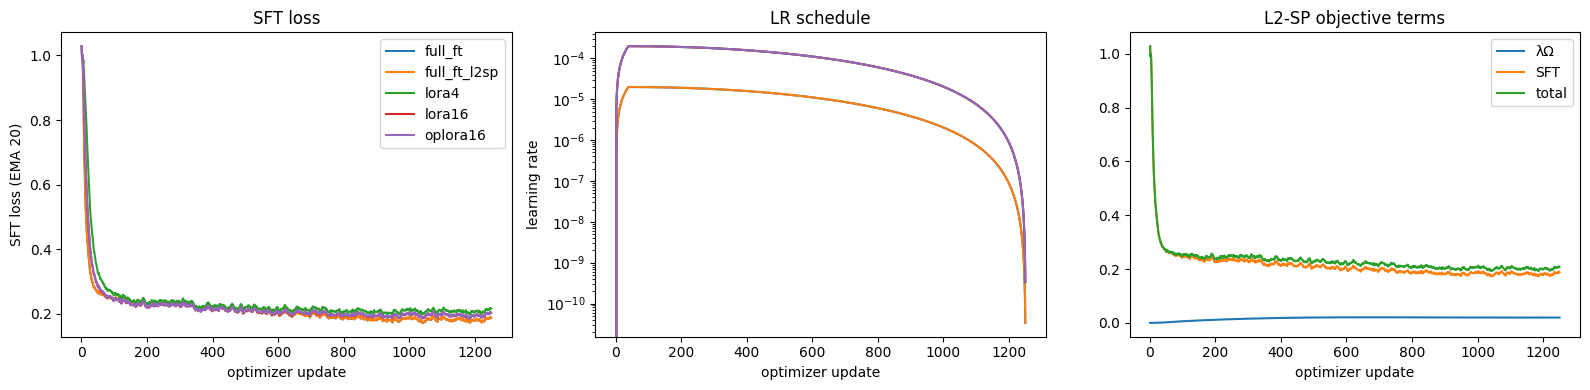
\includegraphics[width=\linewidth]{figs/t1_c17_0.png}
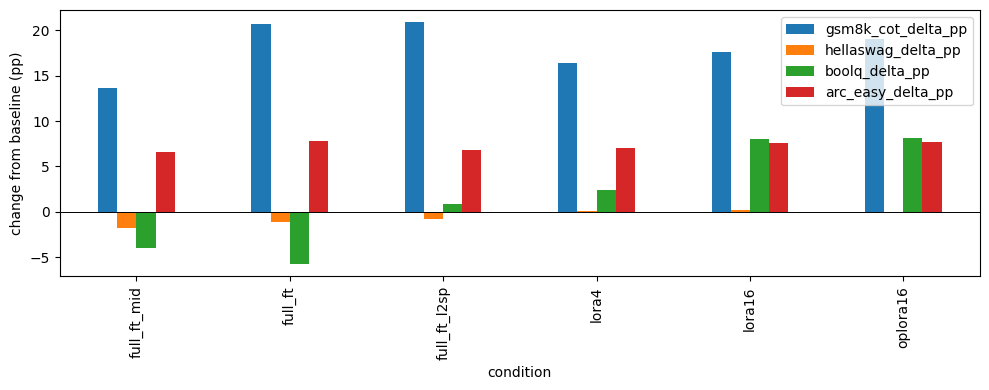
\includegraphics[width=0.62\linewidth]{figs/t1_c17_1.png}
\caption{Task 1. Top: SFT loss, learning-rate schedules (adapters $2{\times}10^{-4}$, Full FT $2{\times}10^{-5}$) and the L2-SP objective terms ($\lambda\Omega$ plateaus near 0.02). Bottom: change from baseline in percentage points for every benchmark and condition.}
\label{fig:t1extra}
\end{figure}

\begin{table}[h]
\caption{Task 3 signal analysis at $N{=}32$ on held-out questions. Spearman correlations are computed within questions and averaged; quartile differences compare correctness in each score's top and bottom quartile within a question (mixed-correctness questions: MATH 469, MathVista 638).}
\label{tab:t3sig}
\centering\small
\begin{tabular}{llrrr}
\toprule
Dataset & Signal & $\rho$(score, length) & $\rho$(score, correct) & top$-$bottom quartile (pp)\\
\midrule
MATH & length $T$ & 1.000 & $-$0.076 & $-$7.8\\
& mean log-prob $L$ & 0.225 & 0.134 & 13.4\\
& self-certainty $K$ & $-$0.161 & 0.198 & 20.4\\
\midrule
MathVista & length $T$ & 1.000 & $-$0.044 & $-$4.5\\
& mean log-prob $L$ & 0.329 & 0.034 & 2.6\\
& self-certainty $K$ & 0.349 & 0.050 & 4.7\\
& visual engagement $V$ & $-$0.686 & 0.036 & 4.3\\
& calibrated confidence $C$ & 0.347 & 0.051 & 5.1\\
& VisConf $Z$ & $-$0.275 & 0.087 & 9.1\\
& tokenwise $Z^\text{tok}$ & $-$0.322 & 0.078 & 8.9\\
\bottomrule
\end{tabular}
\end{table}

\begin{figure}[h]
\centering
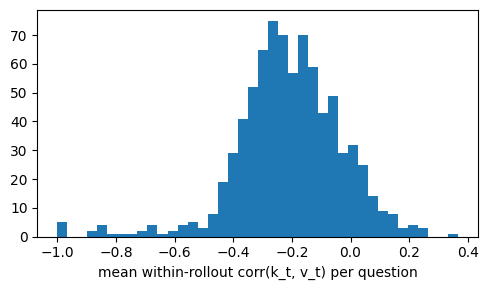
\includegraphics[width=0.30\linewidth]{figs/t3_c8_1.png}\hfill
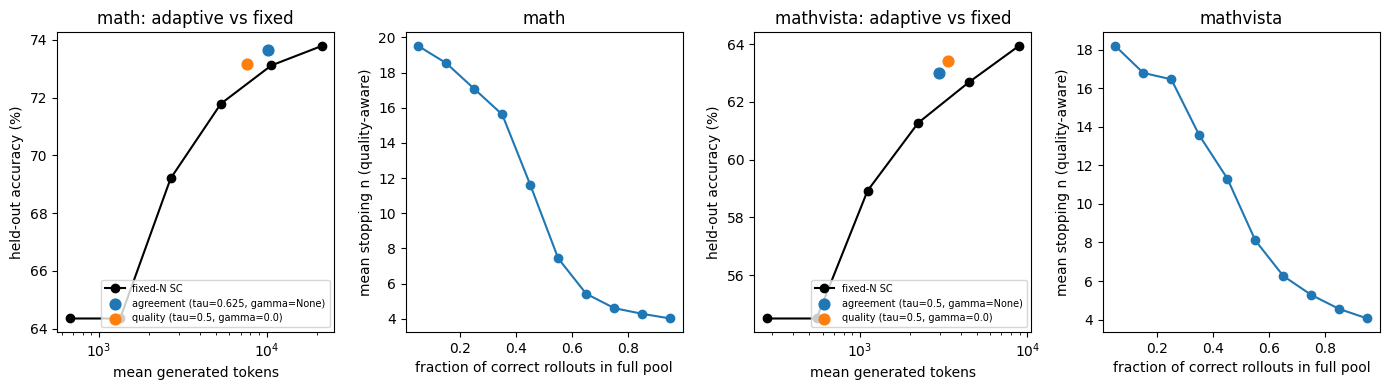
\includegraphics[width=0.66\linewidth]{figs/t3_c12_3.png}
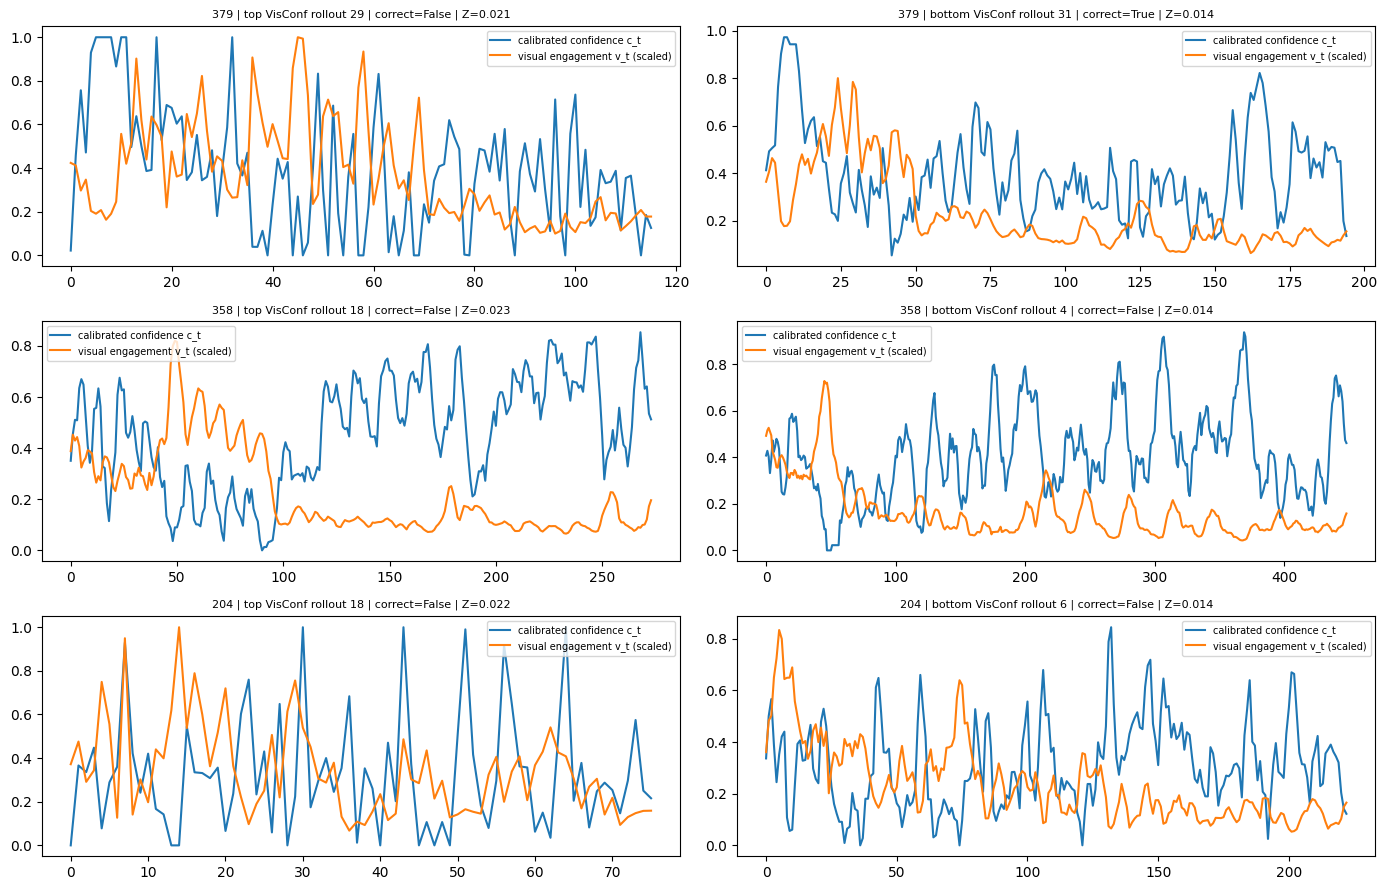
\includegraphics[width=0.85\linewidth]{figs/t3_c8_2.png}
\caption{Task 3. Top left: distribution over questions of the mean within-rollout correlation between token self-certainty and visual engagement. Top right: adaptive vs.\ fixed budgets and mean stopping point of the quality-aware policy against the fraction of correct rollouts in the full pool (retrospective). Bottom: illustrative MathVista trajectories (rule: first three held-out questions where highest-VisConf and self-consistency disagree at $N{=}32$, order 0), calibrated confidence and scaled visual engagement for the top- and bottom-VisConf rollouts.}
\label{fig:t3extra}
\end{figure}

\begin{figure}[h]
\centering
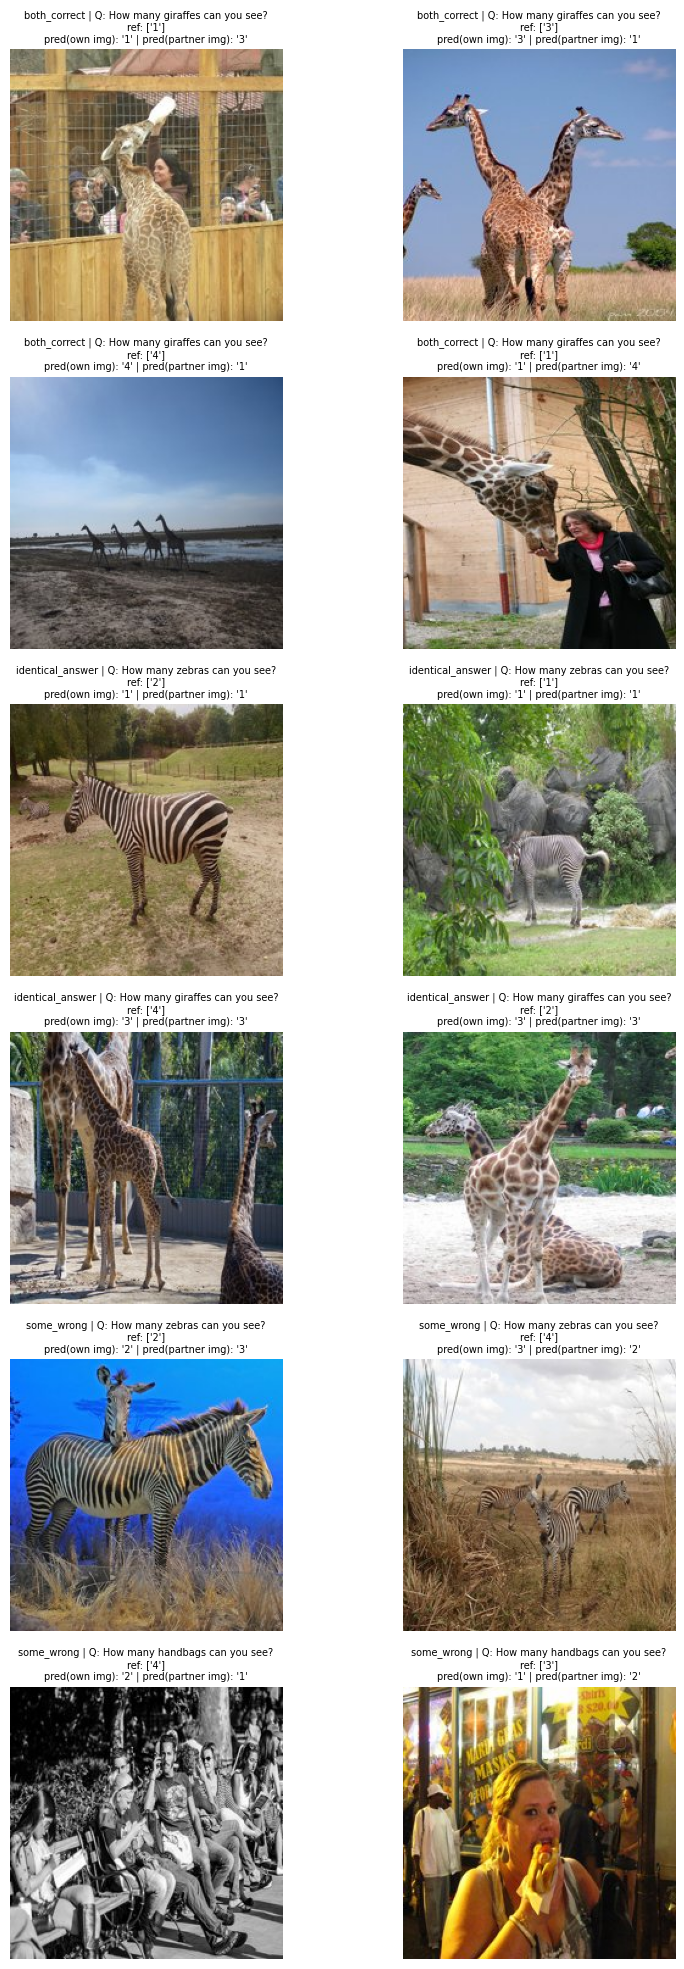
\includegraphics[height=0.45\textheight]{figs/t2_c12_1.png}\hspace{6mm}
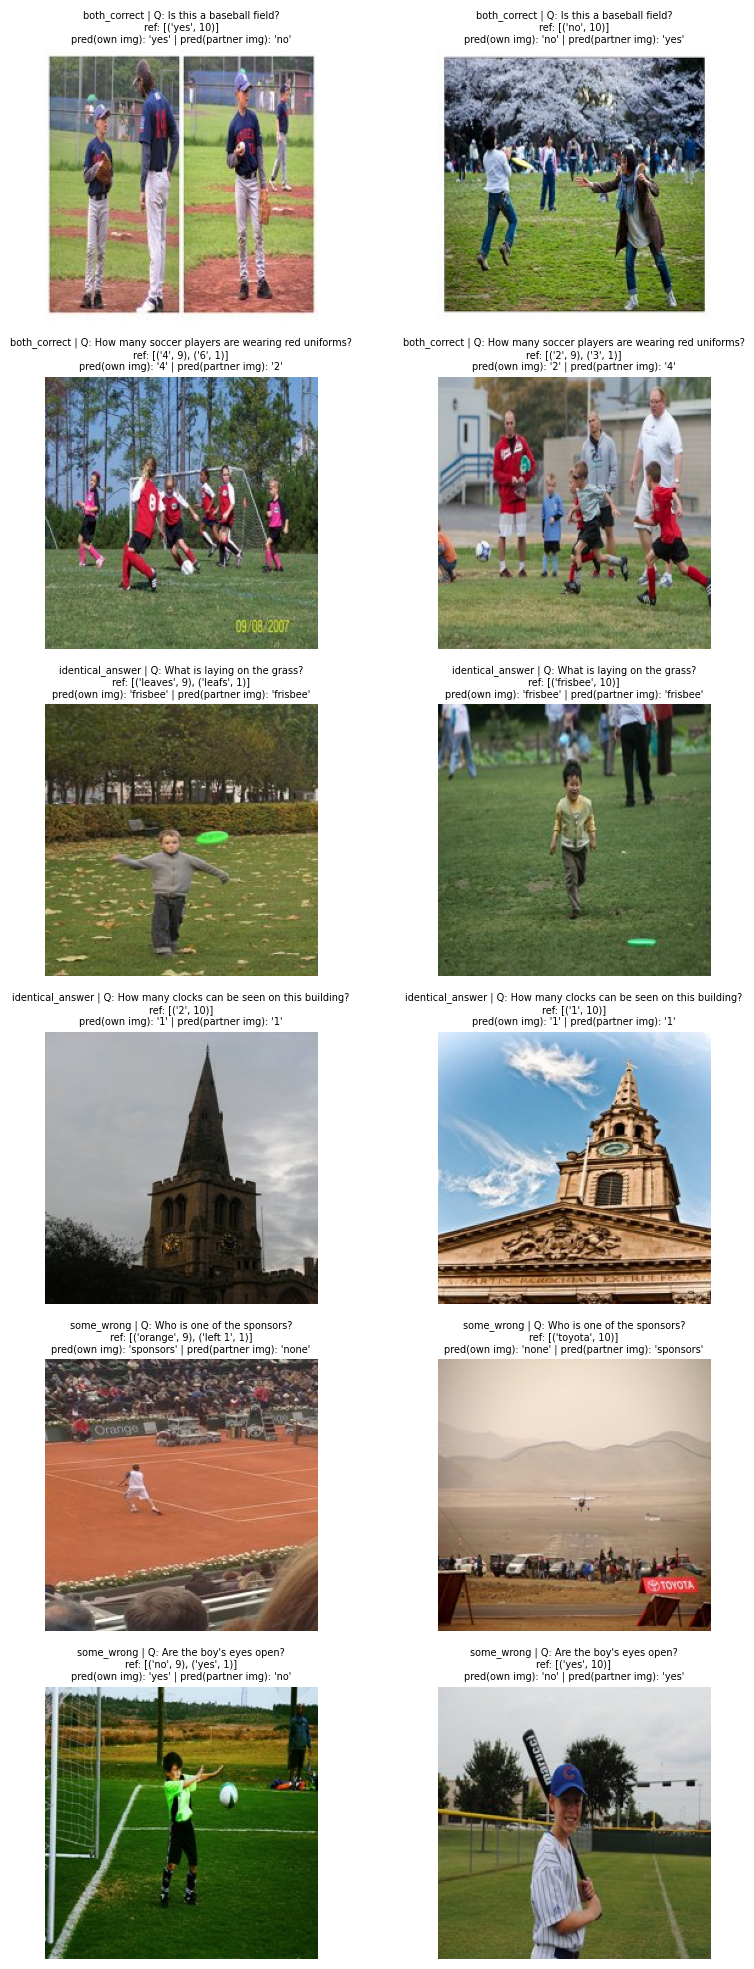
\includegraphics[height=0.45\textheight]{figs/t2_c12_2.png}
\caption{Task 2 complementary pairs (left: template suite; right: VQAv2), showing the shared question, references and greedy predictions with the pair's own and partner image. Selection rule: first two pairs by pair ID in each outcome group (both correct; identical answer for both images; at least one wrong).}
\label{fig:t2qual}
\end{figure}

\end{document}
